% tikz_shapes.tex
% Basic TikZ shapes, colors, fills, and node labels
% Demonstrates fundamental drawing commands in TikZ

\documentclass[12pt,a4paper]{article}

\usepackage{tikz}
\usepackage[margin=1in]{geometry}
\usepackage{amsmath}

% TikZ libraries for advanced features
\usetikzlibrary{shapes.geometric, arrows.meta, positioning, patterns, decorations.pathmorphing}

\title{TikZ Basic Shapes and Drawing}
\author{LaTeX Student}
\date{\today}

\begin{document}

\maketitle

\section{Lines and Basic Shapes}

\subsection{Lines and Paths}

\begin{center}
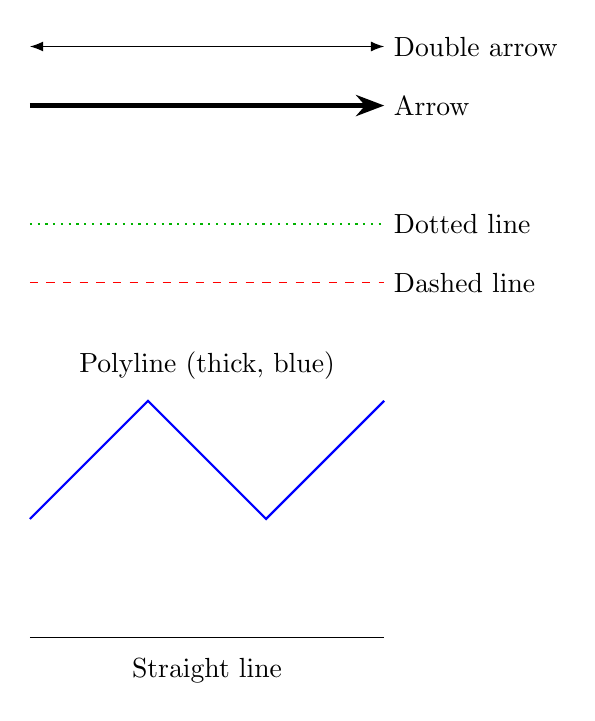
\begin{tikzpicture}[scale=1.5]
    % Simple line
    \draw (0,0) -- (3,0);
    \node[below] at (1.5,-0.1) {Straight line};

    % Line with multiple points
    \draw[thick, blue] (0,1) -- (1,2) -- (2,1) -- (3,2);
    \node[above] at (1.5,2.1) {Polyline (thick, blue)};

    % Dashed and dotted lines
    \draw[dashed, red] (0,3) -- (3,3);
    \node[right] at (3,3) {Dashed line};

    \draw[dotted, green!70!black, thick] (0,3.5) -- (3,3.5);
    \node[right] at (3,3.5) {Dotted line};

    % Line with arrow
    \draw[->, >=Stealth, ultra thick] (0,4.5) -- (3,4.5);
    \node[right] at (3,4.5) {Arrow};

    % Double arrow
    \draw[<->, >=Latex] (0,5) -- (3,5);
    \node[right] at (3,5) {Double arrow};
\end{tikzpicture}
\end{center}

\subsection{Circles and Ellipses}

\begin{center}
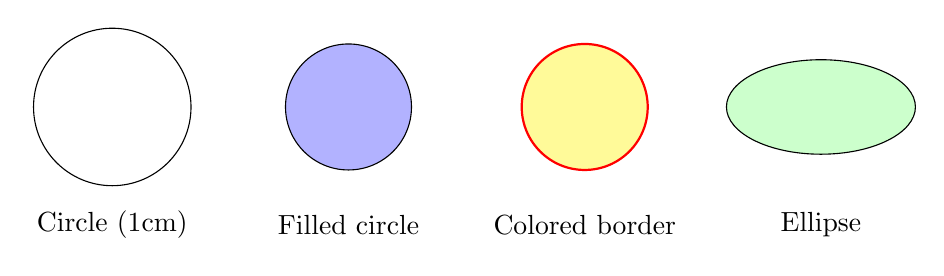
\begin{tikzpicture}
    % Basic circle
    \draw (0,0) circle (1cm);
    \node at (0,-1.5) {Circle (1cm)};

    % Filled circle
    \draw[fill=blue!30] (3,0) circle (0.8cm);
    \node at (3,-1.5) {Filled circle};

    % Circle with colored border
    \draw[draw=red, fill=yellow!40, thick] (6,0) circle (0.8cm);
    \node at (6,-1.5) {Colored border};

    % Ellipse
    \draw[fill=green!20] (9,0) ellipse (1.2cm and 0.6cm);
    \node at (9,-1.5) {Ellipse};
\end{tikzpicture}
\end{center}

\subsection{Rectangles and Squares}

\begin{center}
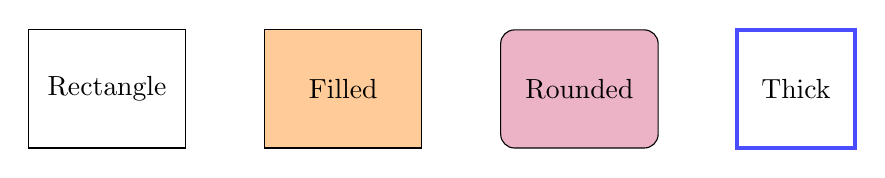
\begin{tikzpicture}
    % Basic rectangle
    \draw (0,0) rectangle (2,1.5);
    \node at (1,0.75) {Rectangle};

    % Filled rectangle
    \draw[fill=orange!40] (3,0) rectangle (5,1.5);
    \node at (4,0.75) {Filled};

    % Rectangle with rounded corners
    \draw[fill=purple!30, rounded corners=5pt] (6,0) rectangle (8,1.5);
    \node at (7,0.75) {Rounded};

    % Square with thick border
    \draw[ultra thick, draw=blue!70] (9,0) rectangle (10.5,1.5);
    \node at (9.75,0.75) {Thick};
\end{tikzpicture}
\end{center}

\section{Arcs and Curves}

\subsection{Arcs}

\begin{center}
\begin{tikzpicture}[scale=1.2]
    % Basic arc
    \draw (0,0) arc (0:90:2cm);
    \node at (0,-0.5) {Arc 0°--90°};

    % Arc with different angles
    \draw[thick, red] (3,0) arc (0:180:1.5cm);
    \node at (3,-0.5) {Arc 0°--180°};

    % Full circle using arc
    \draw[blue, dashed] (7,0) arc (0:360:1cm);
    \node at (7,-0.5) {Arc 360°};
\end{tikzpicture}
\end{center}

\subsection{Bézier Curves}

\begin{center}
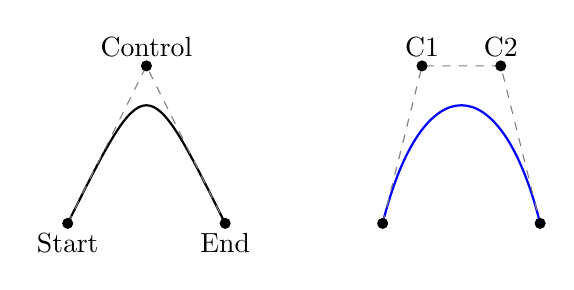
\begin{tikzpicture}
    % Quadratic Bézier curve
    \draw[thick] (0,0) .. controls (1,2) .. (2,0);
    \draw[dashed, gray] (0,0) -- (1,2) -- (2,0);
    \fill (0,0) circle (2pt) node[below] {Start};
    \fill (1,2) circle (2pt) node[above] {Control};
    \fill (2,0) circle (2pt) node[below] {End};

    % Cubic Bézier curve
    \begin{scope}[xshift=4cm]
        \draw[thick, blue] (0,0) .. controls (0.5,2) and (1.5,2) .. (2,0);
        \draw[dashed, gray] (0,0) -- (0.5,2) -- (1.5,2) -- (2,0);
        \fill (0,0) circle (2pt);
        \fill (0.5,2) circle (2pt) node[above] {C1};
        \fill (1.5,2) circle (2pt) node[above] {C2};
        \fill (2,0) circle (2pt);
    \end{scope}
\end{tikzpicture}
\end{center}

\section{Node Labels and Positioning}

\begin{center}
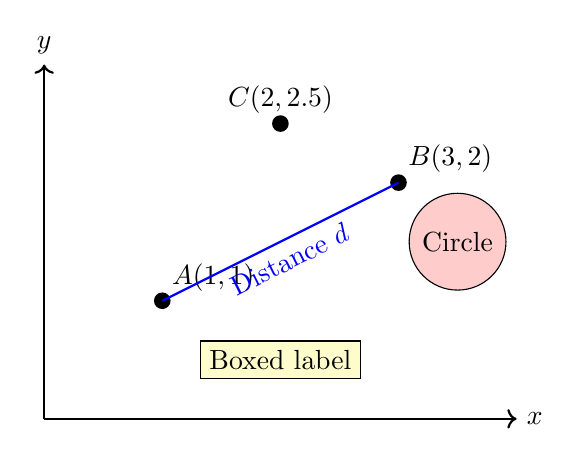
\begin{tikzpicture}[scale=1.5]
    % Nodes with different positions
    \draw[thick, ->] (0,0) -- (4,0) node[right] {$x$};
    \draw[thick, ->] (0,0) -- (0,3) node[above] {$y$};

    % Labeled points
    \fill (1,1) circle (2pt) node[above right] {$A(1,1)$};
    \fill (3,2) circle (2pt) node[above right] {$B(3,2)$};
    \fill (2,2.5) circle (2pt) node[above] {$C(2,2.5)$};

    % Line with midpoint label
    \draw[thick, blue] (1,1) -- (3,2) node[midway, below, sloped] {Distance $d$};

    % Nodes with boxes
    \node[draw, rectangle, fill=yellow!20] at (2,0.5) {Boxed label};
    \node[draw, circle, fill=red!20] at (3.5,1.5) {Circle};
\end{tikzpicture}
\end{center}

\section{Colors and Fills}

\subsection{Color Mixing}

\begin{center}
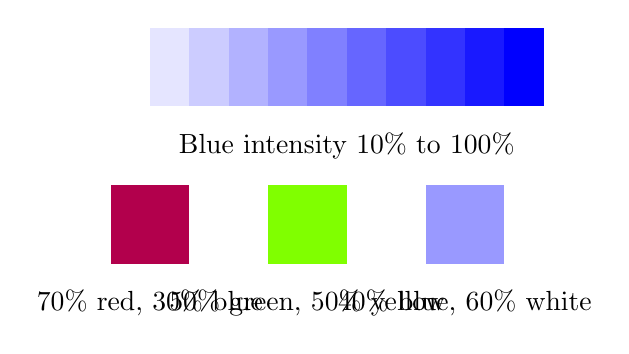
\begin{tikzpicture}
    % Different color intensities
    \foreach \i in {10,20,...,100} {
        \fill[blue!\i] (\i/20,0) rectangle ++(0.5,1);
    }
    \node at (3,-0.5) {Blue intensity 10\% to 100\%};

    % Color mixing
    \begin{scope}[yshift=-2cm]
        \fill[red!70!blue] (0,0) rectangle (1,1);
        \node at (0.5,-0.5) {70\% red, 30\% blue};

        \fill[green!50!yellow] (2,0) rectangle (3,1);
        \node at (2.5,-0.5) {50\% green, 50\% yellow};

        \fill[blue!40!white] (4,0) rectangle (5,1);
        \node at (4.5,-0.5) {40\% blue, 60\% white};
    \end{scope}
\end{tikzpicture}
\end{center}

\subsection{Patterns and Fills}

\begin{center}
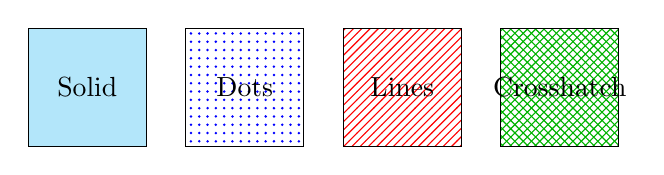
\begin{tikzpicture}
    % Solid fills
    \draw[fill=cyan!30] (0,0) rectangle (1.5,1.5);
    \node at (0.75,0.75) {Solid};

    % Pattern fills
    \draw[pattern=dots, pattern color=blue] (2,0) rectangle (3.5,1.5);
    \node at (2.75,0.75) {Dots};

    \draw[pattern=north east lines, pattern color=red] (4,0) rectangle (5.5,1.5);
    \node at (4.75,0.75) {Lines};

    \draw[pattern=crosshatch, pattern color=green!70!black] (6,0) rectangle (7.5,1.5);
    \node at (6.75,0.75) {Crosshatch};
\end{tikzpicture}
\end{center}

\section{Complex Example: Geometric Shapes}

\begin{center}
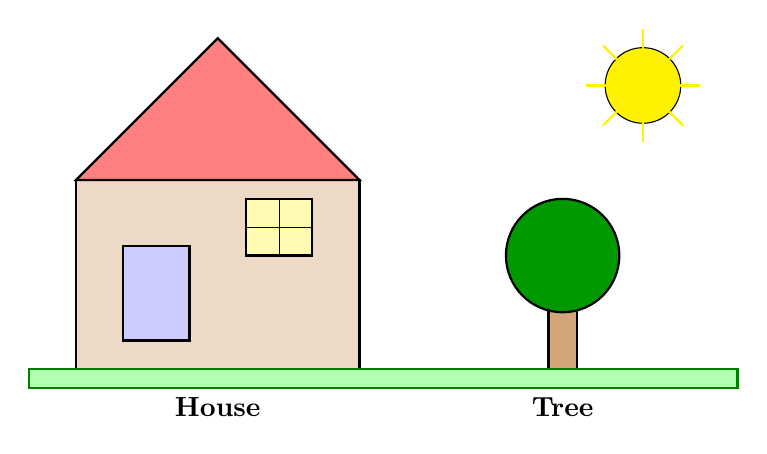
\begin{tikzpicture}[scale=1.2]
    % Draw a house
    \draw[thick, fill=brown!30] (0,0) rectangle (3,2);  % House body
    \draw[thick, fill=red!50] (0,2) -- (1.5,3.5) -- (3,2) -- cycle;  % Roof
    \draw[thick, fill=blue!20] (0.5,0.3) rectangle (1.2,1.3);  % Door
    \draw[thick, fill=yellow!30] (1.8,1.2) rectangle (2.5,1.8);  % Window
    \draw (1.8,1.5) -- (2.5,1.5);  % Window cross
    \draw (2.15,1.2) -- (2.15,1.8);

    % Sun
    \draw[fill=yellow] (6,3) circle (0.4cm);
    \foreach \angle in {0,45,...,315} {
        \draw[thick, yellow] (6,3) -- ++(\angle:0.6cm);
    }

    % Tree
    \draw[thick, fill=brown!70] (5,0) rectangle (5.3,1.2);  % Trunk
    \draw[thick, fill=green!60!black] (5.15,1.2) circle (0.6cm);  % Leaves

    % Ground
    \draw[thick, green!50!black, fill=green!30] (-0.5,-0.2) rectangle (7,0);

    % Labels
    \node[below] at (1.5,-0.2) {\textbf{House}};
    \node[below] at (5.15,-0.2) {\textbf{Tree}};
\end{tikzpicture}
\end{center}

\section{Compilation Notes}

To compile this document:
\begin{verbatim}
pdflatex tikz_shapes.tex
\end{verbatim}

TikZ is processed during the LaTeX compilation, so no additional steps are needed.

\end{document}
